\documentclass[uplatex,dvipdfmx]{jsarticle}
\usepackage{longtable}
\usepackage[uplatex,deluxe]{otf} % UTF
\usepackage[noalphabet]{pxchfon} % must be after otf package
\usepackage{stix2} %欧文&数式フォント
\usepackage[fleqn,tbtags]{mathtools} % 数式関連 (w/ amsmath)

\usepackage{float}
\usepackage{array}
\usepackage{booktabs}
\title{アプリケーション仕様書}
\begin{document}
\maketitle

\section*{1. 利用者向け仕様}
\subsection*{1.1 機能概要}
このアプリは掲示板機能を提供し,利用者は以下の操作を行うことが可能.
まずはじめに「http://localhost:8080/public/bbs.html?」このURLのサイトを開く.実際の画面は図1のようになり,表示されるボタンの種類と説明を表1に示す.
\begin{figure}[H]
\centering
%\vspace{\baselineskip}
%\vspace{-1.5\baselineskip}
 \centering
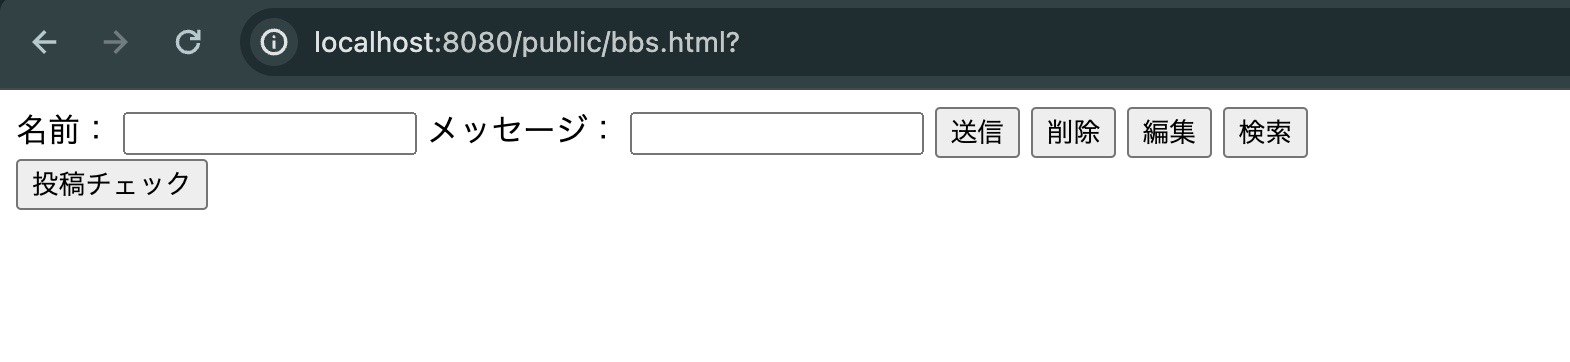
\includegraphics[width=15cm]{ttt.jpg}
%\vspace{\baselineskip}
%\vspace{-1.5\baselineskip}
\caption{実際にWebページを開いた時の画面}
%\vspace{-1.0\baselineskip}
\label{fig:b02}
\end{figure}
\begin{longtable}{|l|l|}
\caption{掲示板の操作ボタンとその機能の説明} \\ % キャプションを上部に配置
\hline
\textbf{ボタン} & \textbf{説明} \\
\hline
\textbf{送信} & 入力した名前とメッセージを掲示板に投稿する \\
\hline
\textbf{削除} & 投稿番号を指定して、該当する投稿を削除する \\
\hline
\textbf{編集} & 投稿番号と新しいメッセージを指定し,投稿を編集する \\
\hline
\textbf{検索} & キーワードを入力し,名前またはメッセージに一致する投稿を検索する \\
\hline
\textbf{投稿チェック} & 全ての投稿を最新の状態で表示する \\
\hline
\end{longtable}

\subsection*{1.2 操作手順}
\begin{enumerate}
\item 名前とメッセージを入力し,「送信」ボタンを押すと新しい投稿が追加される.
\item 「削除」ボタンを押すと,削除したい投稿の番号を入力するダイアログが表示され,指定した番号の投稿が削除される.
\item 「編集」ボタンを押すと.編集したい投稿の番号と新しいメッセージを入力するダイアログが表示され,指定した投稿が更新される.
\item 「検索」ボタンを押すと,キーワードを入力するダイアログが表示され,結果がアラートで通知される.
\item 「投稿チェック」ボタンを押すと,すべての投稿が更新表示される.
\end{enumerate}

\section*{2. 管理者向け仕様}
\subsection*{2.1 サーバーの起動手順}
\begin{enumerate}
\item 任意の場所にディレクトリを作成し,その中に必要なファイル(app8.js,bbs.js,bbs.html,bbs.css)をダウンロードし,配置する
\item ターミナルを開きnode\ app8.jsを実行する
\item 手順2により,サーバーが \texttt{http://localhost:8080} で起動し,リクエストの受け付けを開始する
\item Webページを開き,http://localhost:8080/public/bbs.html?のサイトにアクセスする
\end{enumerate}
\subsection*{2.2各ソースコードの管理}
\begin{itemize}
\item \texttt{app8.js} :サーバー側のロジックを担っており,各種APIのエンドポイント(投稿,削除,編集,検索)を定義している.
\item \texttt{bbs.js} :クライアント側でユーザーの操作を処理しており,fetch APIを用いてサーバーと通信をしている.
\item \texttt{bbs.html} :ユーザーインターフェースを定義している.
\item \texttt{bbs.css} :表示レイアウトとスタイルを管理している.
\end{itemize}
\section*{3. 開発者向け仕様}
\subsection*{3.1 構成ファイル}
\begin{itemize}
\item \texttt{app8.js} : サーバーサイド
\item \texttt{bbs.js} : クライアントサイドの操作スクリプト
\item \texttt{bbs.html} :ユーザーインターフェース
\item \texttt{bbs.css} :レイアウトとスタイルシート
\end{itemize}

\subsection*{3.2 サーバールートと説明}
\begin{longtable}{|l|l|p{8cm}|}
\hline
\textbf{メソッド} & \textbf{ルート} & \textbf{説明} \\
\hline
POST & \texttt{/post} & 新しい投稿を追加する.パラメータ:は\texttt{name}と \texttt{message} \\
\hline
POST & \texttt{/check} & 投稿数を返す. \\
\hline
POST & \texttt{/read} & すべての投稿を取得する.パラメータは\texttt{start} \\
\hline
POST & \texttt{/delete} & 指定した投稿を削除する.パラメータは\texttt{index} \\
\hline
POST & \texttt{/edit} & 指定した投稿を編集する.パラメータは\texttt{index},と\texttt{message} \\
\hline
POST & \texttt{/search} & キーワード検索を行う.パラメータは\texttt{keyword} \\
\hline
POST & \texttt{/like} & 指定した投稿に「いいね」を追加する.パラメータは\texttt{index} \\
\hline
\end{longtable}

\subsection*{3.3 クライアントイベントと対応するサーバー処理}
\begin{longtable}{|l|l|}
\hline
\textbf{イベント} & \textbf{対応するサーバーエンドポイント} \\
\hline
投稿送信 & \texttt{/post} \\
\hline
投稿削除 & \texttt{/delete} \\
\hline
投稿編集 & \texttt{/edit} \\
\hline
投稿検索 & \texttt{/search} \\
\hline
投稿チェック & \texttt{/read} \\
\hline
\end{longtable}

\section*{4. データ形式と例}
\subsection*{4.1 通信フォーマット}
\begin{itemize}
\item \textbf{Content-Type}: \texttt{application/x-www-form-urlencoded}
\end{itemize}

\begin{figure}[H]
\centering
%\vspace{\baselineskip}
%\vspace{-1.5\baselineskip}
 \centering
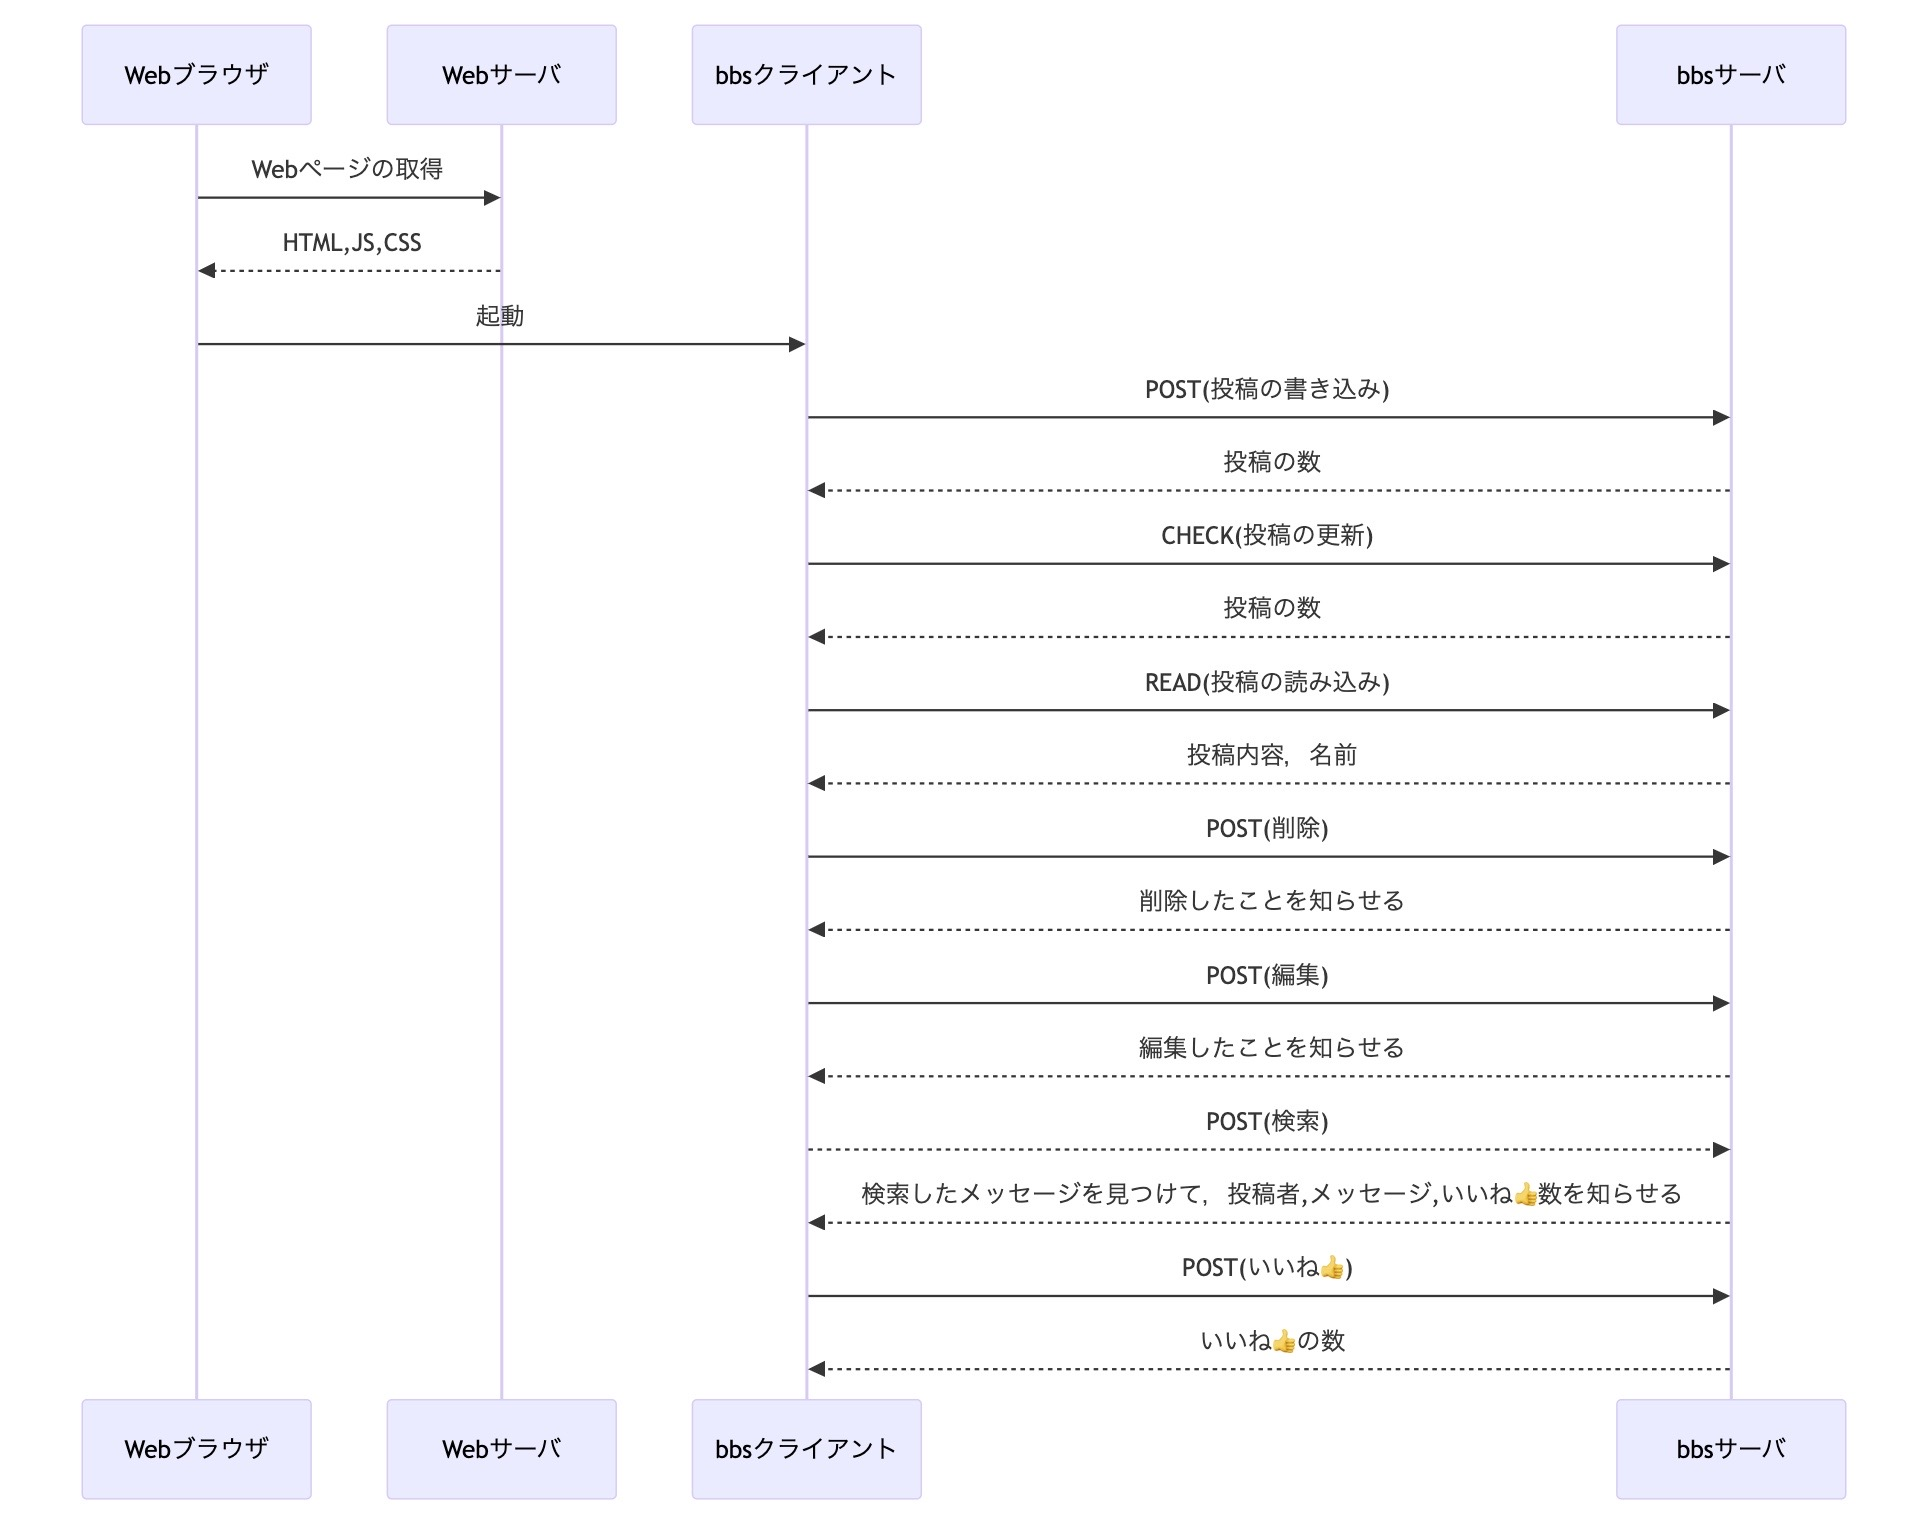
\includegraphics[width=15cm]{rrr.jpg}
%\vspace{\baselineskip}
%\vspace{-1.5\baselineskip}
\caption{Webページの開始,起動,bbsクライアントとサーバのやり取りの全体図}
%\vspace{-1.0\baselineskip}
\label{fig:b02}
\end{figure}

\subsubsection*{POST \texttt{/post}}
\textbf{リクエスト例}
\begin{verbatim}
name=伊藤&message=こんにちは
\end{verbatim}
\textbf{レスポンス例}
\begin{verbatim}
{ "number": 1 }
\end{verbatim}

\subsubsection*{POST \texttt{/read}}
\textbf{リクエスト例}
\begin{verbatim}
start=0
\end{verbatim}
\textbf{レスポンス例}
\begin{verbatim}
{ "messages": [{ "name": "伊藤", "message": "こんにちは", "likes": 0 }] }
\end{verbatim}

\subsubsection*{POST \texttt{/delete}}
\textbf{リクエスト例}
\begin{verbatim}
index=0
\end{verbatim}
\textbf{レスポンス例}
\begin{verbatim}
{ "status": "success", "message": "Deleted successfully" }
\end{verbatim}

\subsubsection*{POST \texttt{/like}}
\textbf{リクエスト例}
\begin{verbatim}
index=0
\end{verbatim}
\textbf{レスポンス例}
\begin{verbatim}
{ "status": "success", "likes": 1 }
\end{verbatim}
\section*{5. Githubリポジトリ}
\end{document}
